\documentclass[../main.tex]{subfiles}
\begin{document}

\chapter{Szyfrowanie treści metodą SDEx (część teoretyczna)}

\section{Opis metody szyfrowania i deszyfrowania SDEx}\label{sec:sdex_encryption_decryption}

Na rysunkach \ref{fig:sdex_encryption_diagram} i \ref{fig:sdex_decryption_diagram} oraz w równaniach \ref{eq:sdex_encryption_equation_block_start} - \ref{eq:sdex_decryption_equation_block_end} użyto oznaczeń:

\begin{itemize}
	\item $ \{M_1,M_2,\ldots, M_i\} $ - bloki tekstu jawnego,
	\item $ \{C_1,C_2,\ldots, C_i\} $ - bloki tekstu zaszyfrowanego,
	\item $ \{h_1,h_2,\ldots, h_k\} $ - dane iteracje hashu,
	\item $ H_{S1} $ - hash z pierwszego klucza sesji,
	\item $ H_{S2} $ - hash z drugiego klucza sesji,
	\item $ H_{S1 \mdoubleplus S2} $ - hash ze złączonych pierwszego i drugiego klucza sesji,
	\item $ \oplus $ - operacja XOR,
	\item $ \mdoubleplus $ - złączenie (konkatenacja) dwóch łańcuchów tekstowych,
\end{itemize}

Szyfrowanie metodą SDEx odbywa się zgodnie z równaniami \ref{eq:sdex_encryption_equation_block_start} - \ref{eq:sdex_encryption_equation_block_end} i ma formę przedstawioną na Rysunku \ref{fig:sdex_encryption_diagram}:

\begin{flalign}
	C_1 &= M_1 \oplus H_{S1} \oplus H_{S1 \mdoubleplus S2} \label{eq:sdex_encryption_equation_block_start} &\\
	C_2 &= M_2 \oplus H_{S1} \oplus H_{S2} &\\
	C_{2k+1} &= M_{2k+1} \oplus h_k \oplus h_{k-1} & \quad k \geq 1 & \quad &\\
	C_{2k+2} &= M_{2k} \oplus H_{S2} \oplus h_{k} & \quad k \geq 1 & \quad &\\
	h_1 &= hash(H_{S1 \mdoubleplus S2}; M_1 \mdoubleplus M_2) &\\
	h_2 &= hash((h_1 \oplus H_{S1 \mdoubleplus S2}); M_3 \mdoubleplus M_4) &\\
	h_k &= hash((h_{k-1} \oplus h_{k-2}); M_{2k-1} \mdoubleplus M_{2k}) & \quad k \geq 3 & \quad  \label{eq:sdex_encryption_equation_block_end}
\end{flalign} 

\begin{figure}[H]
	\centering
	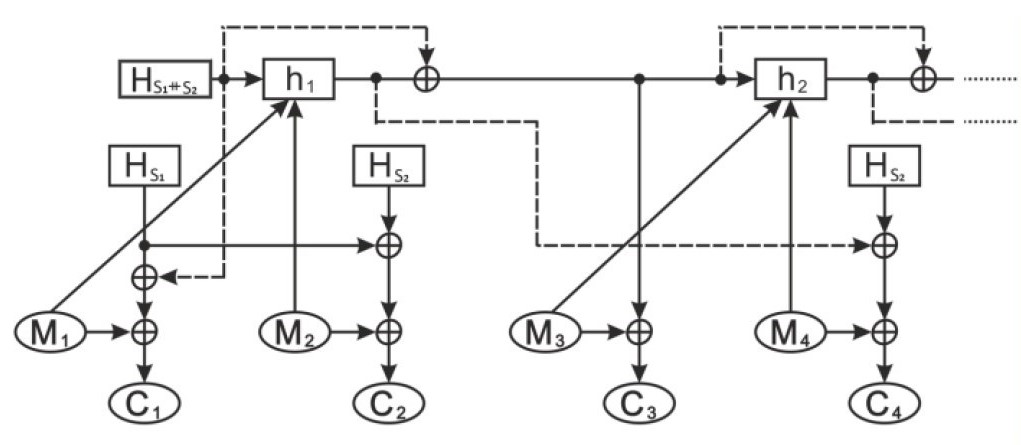
\includegraphics[scale=0.8]{sdex_encryption_diagram.jpg}
	\caption{Diagram algorytmu szyfrowania SDEx}
	\source{dr inż. Artur Hłobaż}
	\label{fig:sdex_encryption_diagram}
\end{figure}

Deszyfrowanie metodą SDEx odbywa się zgodnie z równaniami \ref{eq:sdex_decryption_equation_block_start} - \ref{eq:sdex_decryption_equation_block_end} i ma formę przedstawioną na Rysunku \ref{fig:sdex_decryption_diagram}:

\begin{flalign}
	M_1 &= C_1 \oplus H_{S1} \oplus H_{S1 \mdoubleplus S2} \label{eq:sdex_decryption_equation_block_start} &\\
	M_2 &= C_2 \oplus (H_{S1} \oplus H_{S2}) &\\
	M_{2k+1} &= C_{2k+1} \oplus h_k \oplus h_{k-1} & \quad k \geq 1 & \quad &\\
	M_{2k+2} &= C_{2k} \oplus H_{S2} \oplus h_{k} & \quad k \geq 1 & \quad \label{eq:sdex_decryption_equation_block_end}
\end{flalign} 

\begin{figure}[H]
	\centering
	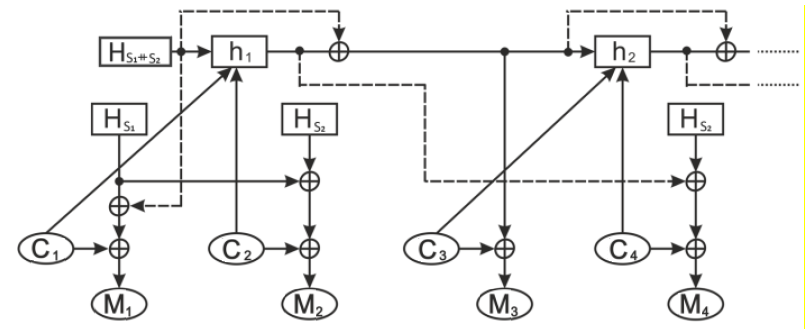
\includegraphics[scale=0.7]{sdex_decryption_diagram.png}
	\caption{Diagram algorytmu deszyfrowania SDEx}
	\source{dr inż. Artur Hłobaż}
	\label{fig:sdex_decryption_diagram}
\end{figure}

Zastosowana została uproszczona metoda SDEx bazująca na publikacji \textit{Analysis of enhanced SDEx method}\cite{sdex_publikacja_2017} po uzgodnieniu z promotorem.

\section{Wybór funkcji skrótu BLAKE 3 do użycia z algorytmem szyfrującym SDEx}

Ze wzorów opisujących proces szyfrowania i deszyfrowania metodą SDEx widać, że głównym czynnikiem decydującym o wydajności algorytmu jest wydajność wykorzystanej funkcji hashującej. Publikacja \textit{Analysis of the Possibility of Using Selected Hash Functions Submitted for the SHA-3 Competition in the SDEx Encryption Method}\cite{sdex_publikacja_2022} przedstawia porównanie efektywności obliczeniowej wybranych popularnych algorytmów hashujących. Wynika z niego, że funkcja skrótu BLAKE 3 oferuje najwyższą wydajność w przeliczeniu na jeden wątek procesora, a także lepszy margines bezpieczeństwa od funkcji hashujących z grupy Grøstl, JH czy Keccak.

\begin{figure}[H]
	\centering
	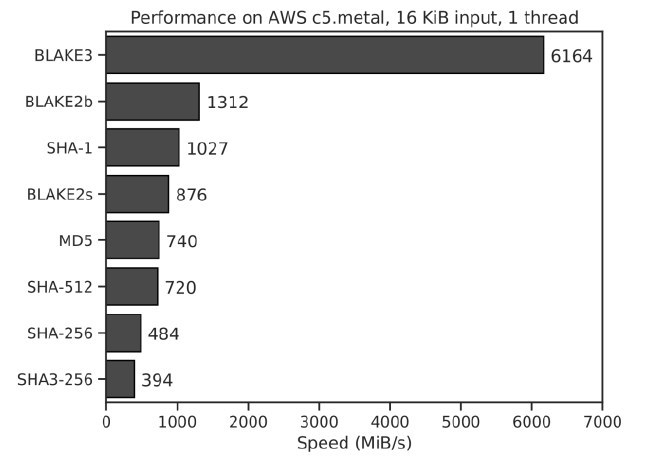
\includegraphics[scale=0.9]{porownanie_wydajnosci_funkcji_hashujacych.jpg}
	\caption{Wydajności obliczeniowe wybranych funkcji skrótu\cite{sdex_publikacja_2022}}
	\label{fig:hash_efficiency_comparison}
\end{figure}

\section{Szyfrowanie i podpisywanie metodą klucza publicznego}

Do nawiązania komunikacji z serwerem, a w dalszej kolejności także wymiany informacji potrzebnych do realizacji szyfrowania i deszyfrowania metodą SDEx potrzebna jest bezpieczna wymiana pewnych informacji między klientem a serwerem oraz między klientami komunikującymi się ze sobą. Do tego celu wykorzystano metodę kryptografii asymetrycznej w oparciu o klucze RSA. Proces komunikacji z użyciem tej techniki kryptograficznej prezentuje Rysunek \ref{fig:asymetric_cryptography_diagram}.

\begin{figure}[H]
	\centering
	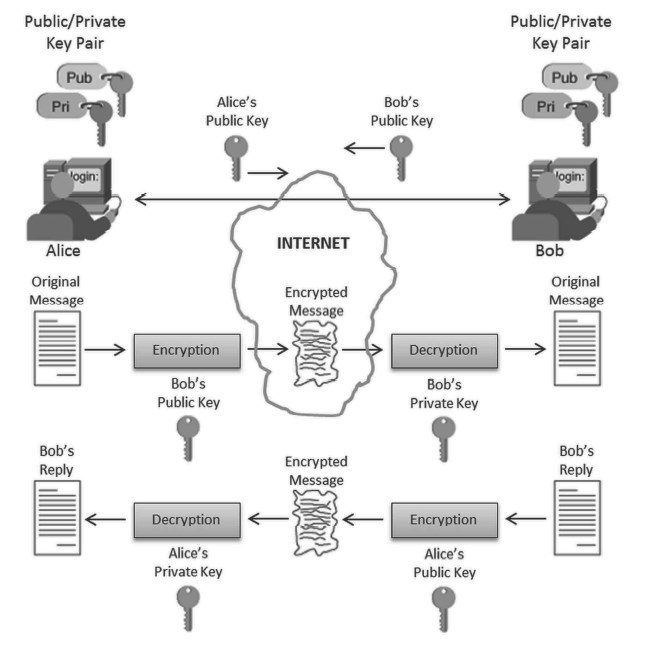
\includegraphics[scale=0.7]{asymetric-cryptography-diagram.jpg}
	\caption{Proces wymiany wiadomości z użyciem kryptografii asymetrycznej\cite{sdex_publikacja_2016}}
	\label{fig:asymetric_cryptography_diagram}
\end{figure}

Z użyciem tej metody wymieniane są między klientami wygenerowane przez nich części klucza sesji $S1$ i $S2$.

Kryptografia asymetryczna umożliwia także podpisywanie wiadomości kluczem prywatnym nadawcy, aby odbiorca mógł zweryfikować autentyczność i niezmienność przyjętej wiadomości. Rysunek \ref{fig:rsa_signing_diagram} przedstawia proces podpisywania wiadomości i jej weryfikacji. W kontekście niniejszej publikacji jest to wykorzystywane do uwierzytelnienia klienta na serwerze.

\begin{figure}[H]
	\centering
	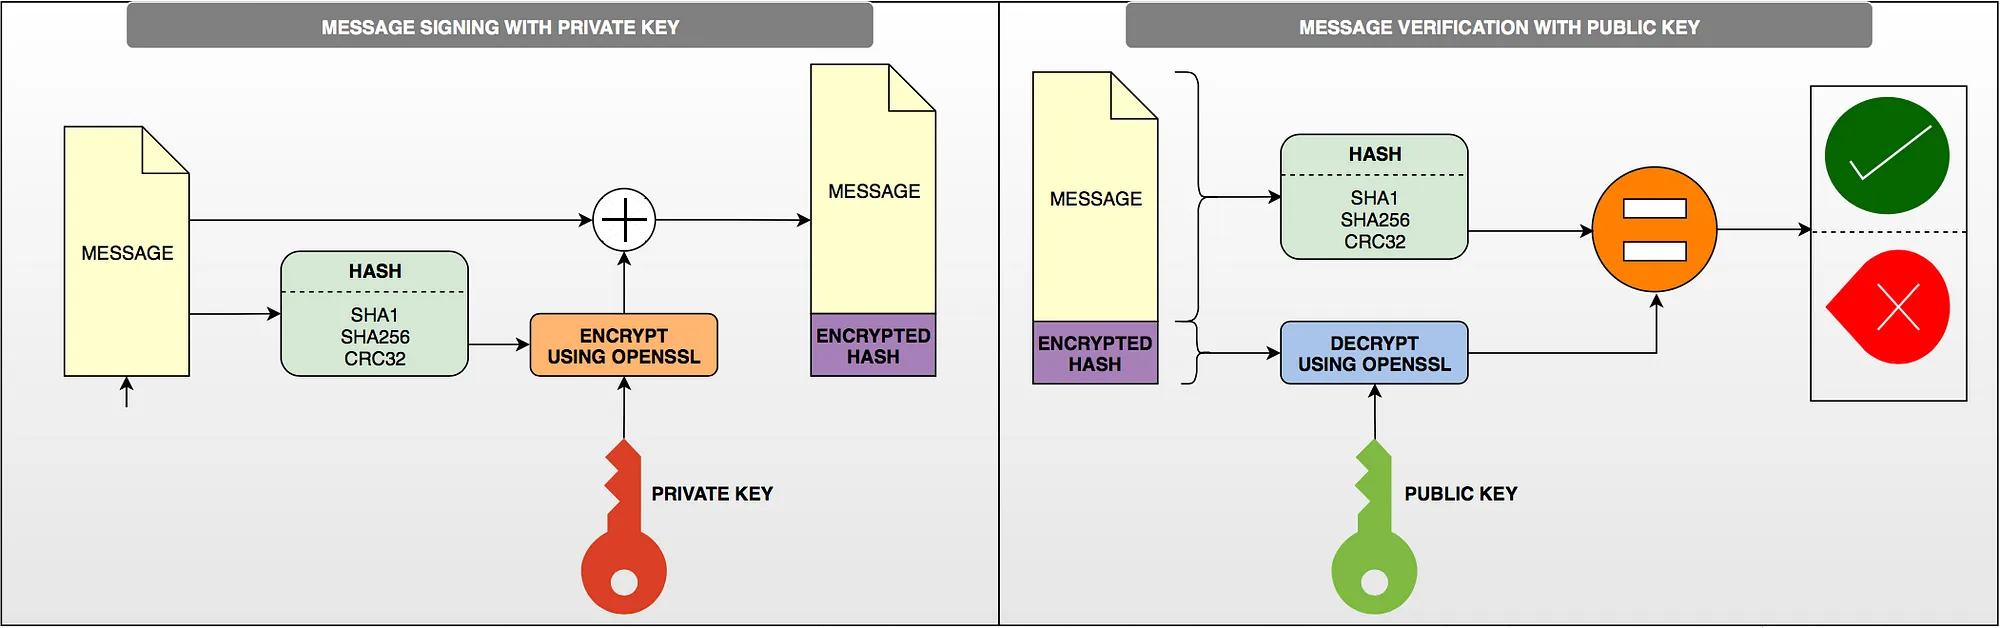
\includegraphics[scale=0.22]{rsa-signing-diagram.jpg}
	\caption{Podpisywanie wiadomości i jej weryfikacja z użyciem kryptografii asymetrycznej\cite{rsa_signing_and_verification}}
	\label{fig:rsa_signing_diagram}
\end{figure}

\section{Rozpowszechnianie kluczy publicznych użytkowników poprzez kody QR}

Klucze publiczne wygenerowane lub wczytywane przez klientów aplikacji, mają wyjściowo formę tekstową, trudną do zapamiętania, a ich rozpowszechnianie metodą kopiowania i wklejania jest mało atrakcyjne dla użytkowników (w porównaniu przykładowo do wymiany numerów telefonów, które są krótsze i łatwiejsze do krótkotrwałego zapamiętania dla człowieka) oraz podatne na błędy, gdyż zawierają one znaki nowej linii, w tym znak nowej linii na końcu tekstu klucza, który łatwo przeoczyć przy kopiowaniu, co może powodować błąd przy próbie zaszyfrowania wiadomości takim niepełnym kluczem.

Wybraną metodą rozpowszechniania kluczy publicznych jest zakodowanie ich do postaci kodu QR. Posiadają one bardziej atrakcyjną wizualnie formę obrazka, który łatwo można udostępnić na przykład na platformie społecznościowej, a także umożliwiają klientowi w prosty sposób wykorzystanie go, aby dodać klucz publiczny innego użytkownika poprzez zeskanowanie obrazka aparatem w telefonie lub wczytanie go z pamięci telefonu. Ponadto standard kodu QR zapewnia korekcję błędów do nawet 30\% zakodowanej zawartości\cite{qr_code_erorr_correction}.

Wymianę kluczy publicznych tą metodą w oparciu o platformę społecznościową przedstawiają rysunki \ref{fig:qr_codes_exchange_diagram} oraz \ref{fig:qr_codes_exchange_diagram_2}.

\begin{figure}[H]
	\centering
	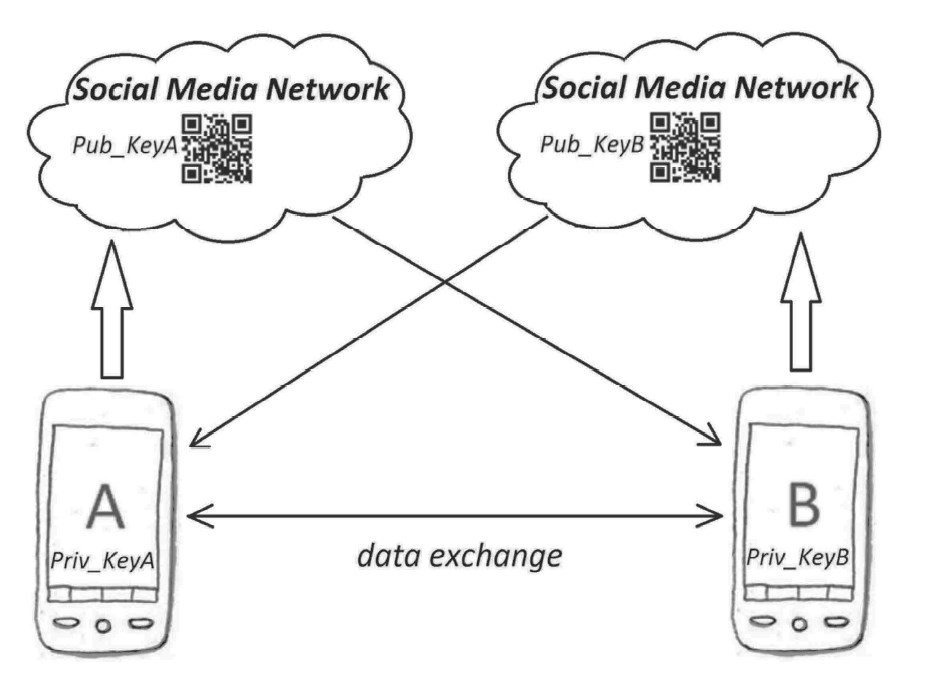
\includegraphics[scale=0.5]{exchanging-qr-codes-diagram.jpg}
	\caption{Wymiana kodów QR z kluczami publicznymi w oparciu o platformę społecznościową\cite{sdex_publikacja_2016}}
	\label{fig:qr_codes_exchange_diagram}
\end{figure}
\vfill

\begin{figure}[H]
	\centering
	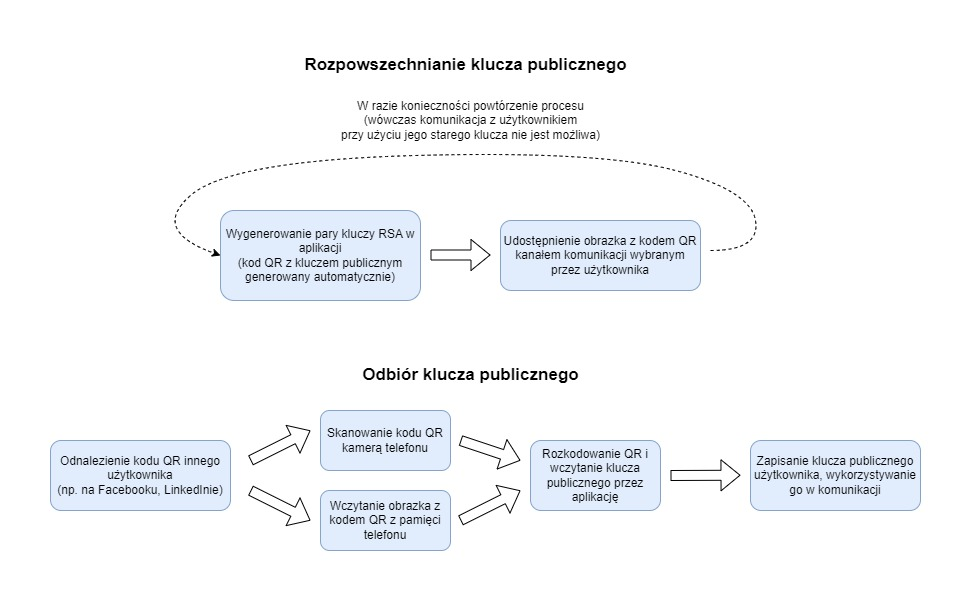
\includegraphics[scale=0.46]{exchanging-qr-codes-diagram-2.jpg}
	\caption{Wymiana kodów QR z kluczami publicznymi}
	\source{opracowanie własne}
	\label{fig:qr_codes_exchange_diagram_2}
\end{figure}

\section{Wybór technologii do realizacji części praktycznej pracy}\label{sec:application_technology_choices_theory}

\subsection{Technologie aplikacji mobilnej}

W celu realizacji niniejszej pracy potrzeba było stworzyć aplikację mobilną uruchamianą na telefonie komórkowym (smartfonie). Istnieje wiele popularnych technologii umożliwiających stworzenie takiego oprogramowania, które dawałyby możliwość implementacji założeń opisanych w sekcji \ref{sec:mobile_application_requirements}. Technologie te można podzielić na natywne (\textit{native apps}), natywne między platformowe (\textit{native cross-platform}), sieciowe (\textit{web apps}), progresywne aplikacje sieciowe (\textit{progressive web applications}, PWA) oraz łączące cechy aplikacji natywnych i sieciowych - czyli hybrydowe\cite{mobile_applications_typology}\cite{mobile_applications_typology_2}.

Aplikacje natywne z reguły są wydajniejsze i bardziej energooszczędne od ich webowych odpowiedników\cite{android_vs_web_energy_efficiency_comparison}, a do tego oferują pełniejszy dostęp do funkcjonalności urządzenia, na którym pracują (na przykład możliwość korzystania z kamery urządzenia, jego pamięci masowej czy wbudowanej szyfrowanej bazy danych do przechowywania certyfikatów i haseł).

Istotną kwestią przy wyborze technologii jest także dojrzałość danego "ekosystemu", czyli dostępność bibliotek ułatwiających tworzenie oprogramowania, aktualność i zgodność tych bibliotek ze współczesnymi standardami bezpieczeństwa oraz aktualnymi wersjami interfejsów programowania aplikacji (ang. \textit{application programming interface}, API) zgodnymi z nowszymi wersjami systemów operacyjnych, na których działają współczesne telefony, a także dostępność narzędzi wspomagających procesy testowania, debugowania i budowania aplikacji.

Do realizacji części praktycznej niniejszej pracy wykorzystany został framework React Native umożliwiający tworzenie natywnych aplikacji między platformowych. Z użyciem tego frameworka kod napisany w języku JavaScript jest kompilowany do kodu natywnego dla platformy docelowej\cite{react_native}, co przy wzięciu pod uwagę pewnych różnic wynikających z odmienności platform mobilnych (różne funkcjonalności oraz niejednolite API tych platform) pozwala stworzyć kod działający na urządzeniach różnych producentów w sposób jednakowy lub zbliżony.

Do wyboru tej technologii przyczyniły się:
\begin{itemize}
	\item szeroka dostępność bibliotek,
	\item wsparcie i rozwój tej technologii przez rozpoznawalną i doświadczoną w branży IT firmę (Meta),
	\item możliwość tworzenia natywnych modułów pisanych w językach właściwych dla danej platformy (dla Androida jest to Java i Kotlin, dla iOS - Swift oraz ObjectiveC), co w przypadku braku implementacji pewnych funkcji tych platform w ramach frameworka i bibliotek umożliwiałoby ich własnoręczne zaimplementowanie),
	\item wydajność aplikacji tworzonych z użyciem tego frameworka jest zbliżona do aplikacji tworzonych w językach natywnych dla wybranej platformy (np. w Javie)\cite{android_vs_react_native_performance_comparison},
	\item rozpowszechniająca się adopcja React Native w produktach komercyjnych\cite{reacti_native_use_statistics}
\end{itemize}

\subsection{Wybór technologii backendowej do implementacji aplikacji serwerowej}

Do realizacji aplikacji serwerowej należało wybrać technologie umożliwiające zarówno komunikację webową (za pośrednictwem websocketów) z klientami mobilnymi, jak również mogącą komunikować się z bazą danych, co wynika z założeń funkcjonalnych opisanych w sekcji \ref{sec:backend_application_requirements}.

Istotną kwestią przy wyborze tych technologii była obsługa asynchronicznej komunikacji z pojedynczym oraz z wieloma klientami. Również dla aplikacji serwerowej istotnym czynnikiem była dostępność bibliotek, które implementują wymagane funkcjonalności oraz aktywny rozwój przez ich autorów. Ze względu na te wymagania, a także wcześniejszą dobrą znajomość tych technologii przez autora niniejszego opracowania wybrany został język Python oraz framework FastAPI działający na serwerze Uvicorn. Na ten wybór wpłynęła przede wszystkim leżąca u podstaw frameworka FastAPI i prosta w programowaniu asynchroniczność obsługi żądań (requestów), rozwiązania bazujące na aktualnych standardach języka Python oraz dość wysoka wydajność tego frameworka i Uvicorna\cite{fastapi_performance}. Korzyścią wynikającą z wyboru języka Python jest fakt, że posiada on wbudowane w bibliotekę standardową wsparcie dla bazy danych SQLite, która została wykorzystana do przechowywania danych o klientach.

\subsection{Wybór protokołu łączności klientów mobilnych z serwerem}

Przy wyborze protokołu łączności między urządzeniami klientów a serwerem brano pod uwagę protokół HTTP z architekturą REST (ang. \textit{representational state transfer}) i protokół WebSocket. Po przeanalizowaniu wymagań funkcjonalnych, jakie musi spełniać aplikacja oraz różnic w zastosowaniu tych rozwiązań\cite{rest_vs_websockets}\cite{rest_vs_websockets_2} jednoznacznie wybrana została komunikacja w oparciu o protokół WebSocket. Przede wszystkim WebSocket lepiej nadaje się do obsługi komunikacji wywołanej zdarzeniami (\textit{event-based}), która jest typowa dla aplikacji typu czat. Dzięki temu można w prosty sposób zaimplementować przekazywanie wiadomości w obie strony (full-duplex), to jest od klienta do serwera i odwrotnie, a także trójstronną komunikację (klient 1 - serwer - klient 2), a przy tym z minimalnymi opóźnieniami pomiędzy wysłaniem i doręczeniem wiadomości. Chcąc odwzorować ten mechanizm w oparciu o protokół HTTP trzeba byłoby wykonywać cykliczne zapytania do serwera w krótkich odstępach czasu, aby uzyskać informacje zwrotne z przebiegu komunikacji.

\end{document}